\section{(ゲーム体験版・デモムービーの)ミラーサイトやってみた!}

\subsection{はじめに}
はじめまして。@ijust3\footnote{https://twitter.com/ijust3}と申します。普段は会社で家電向けのクライアント・アプリケーション開発をしておりますが、本日はWebサービスの話題で書きます。

ゲームの体験版やデモムービーをダウンロードする際に、時々見かけるミラーサイト。そういえば、いつも似たようなサイト名やサイトバナーが並んでいるような。皆様も気になりませんか?(図\ref{fig:mirrors})

そんなちょっとした興味が切っ掛けとなり、2009年から「Magic Mirror」というサイト名でゲーム関連のミラーサイトの運営を行ってみました。\footnote{http://magics.ddo.jp/}

今は仕事が忙しくサイトの更新が滞っているのですが、最盛期で一日平均5,6個のファイルの追加を行っていました\footnote{月曜から木曜まではおよそ1日1個から数個、金曜日から土曜日が素材の更新が最も多くなります。}。PVは一日3000から5000です。

\begin{figure}[hbp]
 \begin{center}
  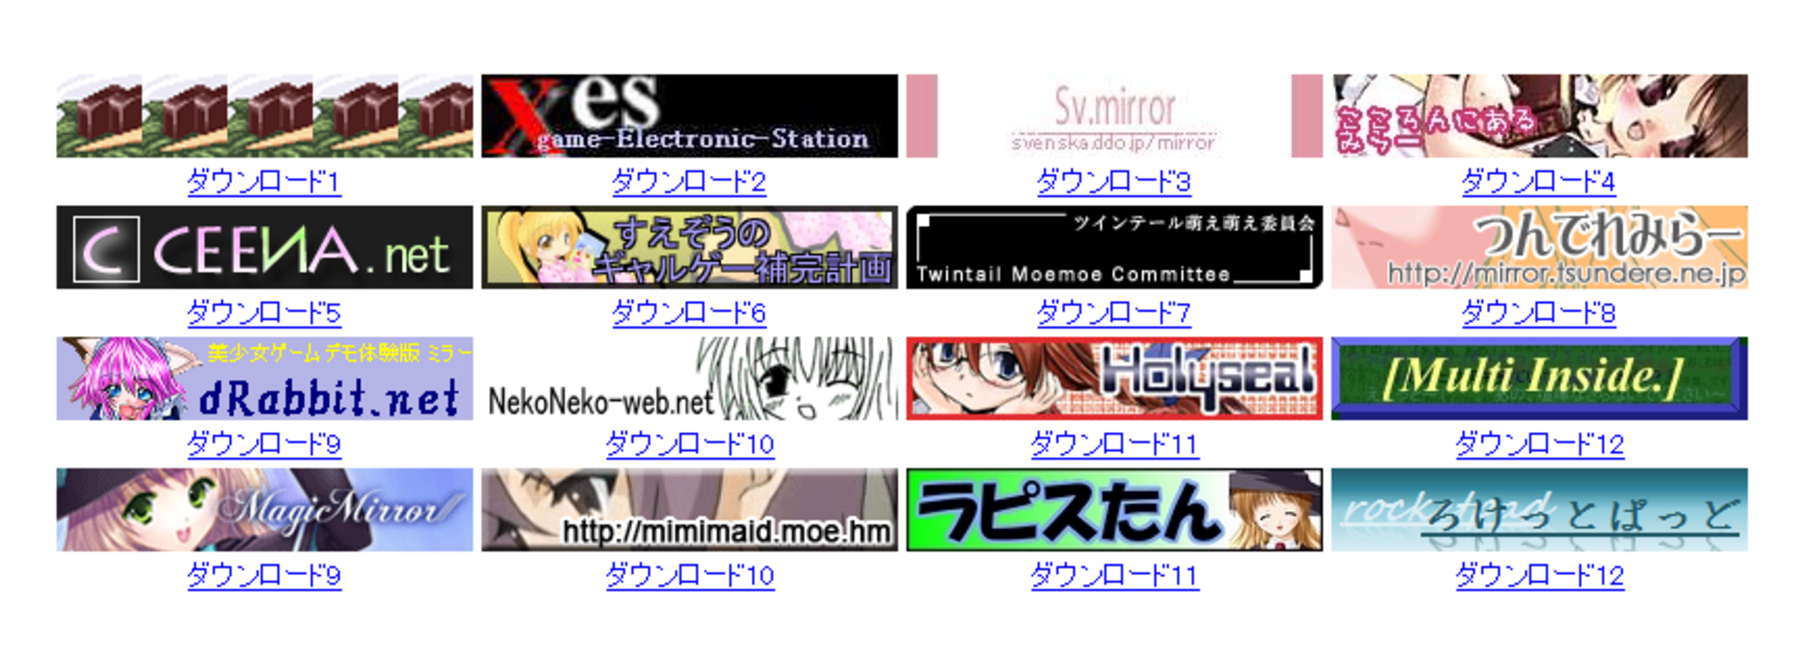
\includegraphics[width=110mm]{ijust3-mirror/img/mirrors.eps}
 \end{center}
 \caption{ミラーサイトへ貼られたダウンロードリンク}
 \label{fig:mirrors}
\end{figure}

\subsubsection{ミラーサイトとは}

ゲーム関連のミラーサイトとは、ゲームメーカーや同人のゲームサークルが配布するゲームの体験版、デモムービー、主題歌、壁紙、チラシ、ドラマCD、ラジオ音声、ゲーム本体\footnote{無料の同人ゲームやミニゲームなど}、パッチなどの素材である配布データを複製し、再配信を行っているサイトのことです。%
ネット上にはこの種のミラーサイトは複数存在します。そのサイトはすべて有志で運営されています。
%なお、ゲームメーカ等の公式サイトでも、ダウンロードページで「ミラーサイト」の表記\footnote{他にも「ダウンロード支援サイト」、「協力サイト」等の表記がされることもあります}が使用されていることが少なくありません。

\subsubsection{個人ミラーサイトの歴史}
個人ミラーサイトの歴史についてはmirror.fuzzy2.comさんが簡潔にまとめています。\cite{fuzzy2_1}

要約すると、ブロードバンド回線が一般的になり、多くのユーザがゲームメーカーのサイトから配布している素材のダウンロードをするようになりました。そのため、メーカー側のサーバの能力の限界に達し、しばしばダウンする事態になりました。この問題に対して、「ユーザーによる継続的な支援」の一つが個人ミラーサイトです。ミラーといってもメーカーからの許諾を得ず配布を行ってしまうと問題があります。2002年頃から一部の個人ミラーサイト間で連携が始まり、J-NODEという流通メーカーの担当者が中心となって、メーカーや流通会社へ個人ミラーサイトがミラーの許諾を得るための仕組みができていきました。そのJ-NODEの担当者の退職に伴い、その参加メンバーが中心となって「KEL有志ミラー」を結成。当時J-NODEのメーリングリストがJDMという名称だったことからアルファベットを一文字進めてKELとなりました。\cite{XES}


\subsubsection{KEL有志ミラー}

「KEL有志ミラー」はゲームソフト関連の素材をミラーするサイトの集まりです。Magic Mirrorも例外ではなく「KEL有志ミラー」参加サイトと連携をしながら活動を行っています。

有志のメンバーは、ミラーサイトの管理者で構成されています。

\subsubsection{素材の用意}

一般的なミラーの流れとして、メーカーがミラーを希望する場合、メーカーから依頼の連絡がきます。体験版などの素材が公開日の1-2日前に届き\footnote{かなり余裕を持って素材が届くこともあるが、差し替えが発生することを見越して皆、数日前まで何もしないことも多い}、各ミラーサイトは公開の準備をすることになります。%
過去にミラーを行ったことのあるメーカー・サークルには、引き続き同じミラーサイト管理者が連絡窓口を担当することが多く\footnote{幹事と呼ばれます}、%
もしメーカーから依頼がなかった場合は、その幹事がメーカーにミラーをさせて欲しいと許諾申請をします。\footnote{或いは特定の範囲の素材について事後報告でミラーを行なっても良い旨、転載許諾を事前に取得している場合もあります。}%
新規のメーカーの場合は、その時々に応じて幹事が選任されます。\footnote{ブランドが独立した場合等は例外もあります。}。%
また、新しくできた同人サークルからの依頼があった場合は、その依頼を最初に有志ミラーへ報告したサイトが、そのサークルの担当となる場合が多いです。\cite{XES}

例外も多々あり、例えばメーカによっては各ミラーサイトが個別に連絡を取らないとミラーの許諾を貰えないという場合等は良くあります。

\subsubsection{活動と目的}
各々のミラーサイトの活動は、独自色を持つサイトも多く、多岐に渡りますが、単純に「素材の再配信」だけを考える場合、ミラーサイトの活動と目的は次の2つに分類出来ます。\cite{fuzzy2_2}
\begin{enumerate}
 \item 負荷分散\\
  負荷分散をするため、各ミラーサイトで再配信を行います。
  古くから存在するミラーサイトのmirror.fuzzy2.comさんが指摘されるように、現在でも人気の高いファイルは公開直後から数週間程の間、大量のアクセスがかかります\cite{fuzzy2_1}
  図\ref{fig:download-graph}はその一例として前作がアニメ化された人気タイトルが去年11月に体験版を出した際のダウンロード数を日次で集計したものですが、公開直後の2週間程度で比較的多めのアクセスが続き、その後アクセスが落ち着いて行く様子が見て取れます。\footnote{休日やその前日等にアクセスが増えるため、グラフは山なりになっています}

 \item 転載\\
  負荷分散以外の様々な理由で、ミラーサイト側からメーカーへ許諾を取り、再配信を行います。
  例えば、メーカーがデモムービーを動画共有サービスのみで公開を開始するような時に、メーカーへ確認を取り、ミラーサイトでユーザが素材をダウンロード出来るようにする等の場合があります。
\end{enumerate}

\begin{figure}[htbp]
 \begin{center}
  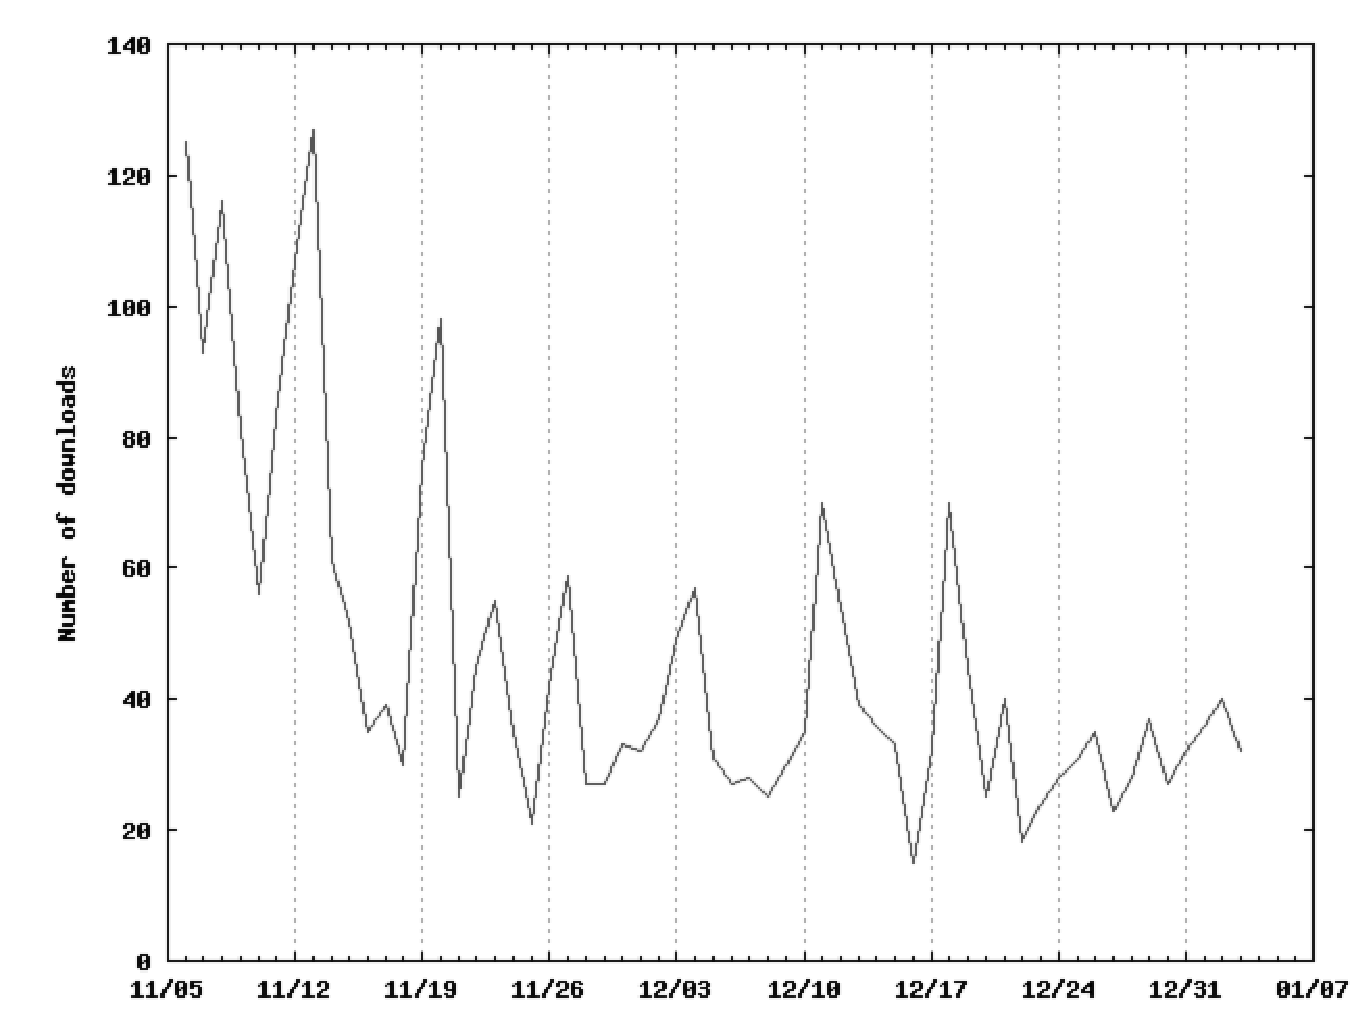
\includegraphics[width=110mm]{ijust3-mirror/img/download-graph.eps}
 \end{center}
 \caption{ある商業作品体験版のミラー公開後のダウンロード数の推移}
 \label{fig:download-graph}
\end{figure}

\subsubsection{KEL有志メンバーになるには}

私の場合はミラーサイトの土台だけ作り\footnote{はりぼて...}、KEL-mirror MLの管理者である「まるちいんさいど」さん\footnote{\url{http://www.pachi.ac/~multi/index.shtml}}へ連絡をしました。%
KEL-mirror MLへ参加し、その後、ミラーサイトの基準を満たしているか確認\footnote{転載禁止の表記や、ミラーサイトで扱う素材によってはR18のゾーニング分けが出来ているかどうか等}をして頂きました。基準をパスし、ミラーサイトを開始しました。

\subsubsection{ミラー開始までの流れ}

素材のミラーが開始されるまでの流れはだいたいこんな感じです。\cite{XES}
\begin{enumerate}
 \item メーカーやサークルからのミラーの依頼、またはKEL側のメーカ-・サークル毎に割り振られた担当者(幹事と呼ばれる)が許諾申請
 \item KEL有志ミラーメーリングでの募集・情報公開
 \item 各ミラーサイトでのファイルの取得・設置
 \item 幹事がメーカー・サークルへミラーを行ったサイトの情報を報告
 \item ミラー公開
\end{enumerate}

% -------------------------- 技術編 ------------------------------

\subsection{運用環境}
本節では、MagicMirrorで使用している運用環境について紹介します。

\subsubsection{サーバ構成}

\begin{itemize}
 \item VPS - Webサーバ + DBサーバ 
 \item VPS - ファイルサーバ(アクセスが集中する素材の置き場所)
 \item 自宅 - ファイルサーバ(アクセスが集中しない素材の置き場所)
\end{itemize}

ミラーサイトの基本はWebでファイルを公開することです。

MagicMirrorのサーバは3台あります。1台はミラーサイトのWebサーバと、DBサーバです。扱っているミラー素材の索引・検索・ダウンロードページなどを提供しています。もう2台はファイルサーバとなっていて、VPSは30G程度で、自宅サーバのストレージは4T程度です\footnote{1Tバイトのハードディスクを4つ使っていますがRAID構成ではなく、そのままつかっています。データが消えても補完できるためです}。最近ではギガ単位の素材も増えてきましたが、しばらくは大丈夫そうです。

\begin{figure}[htbp]
 \begin{center}
  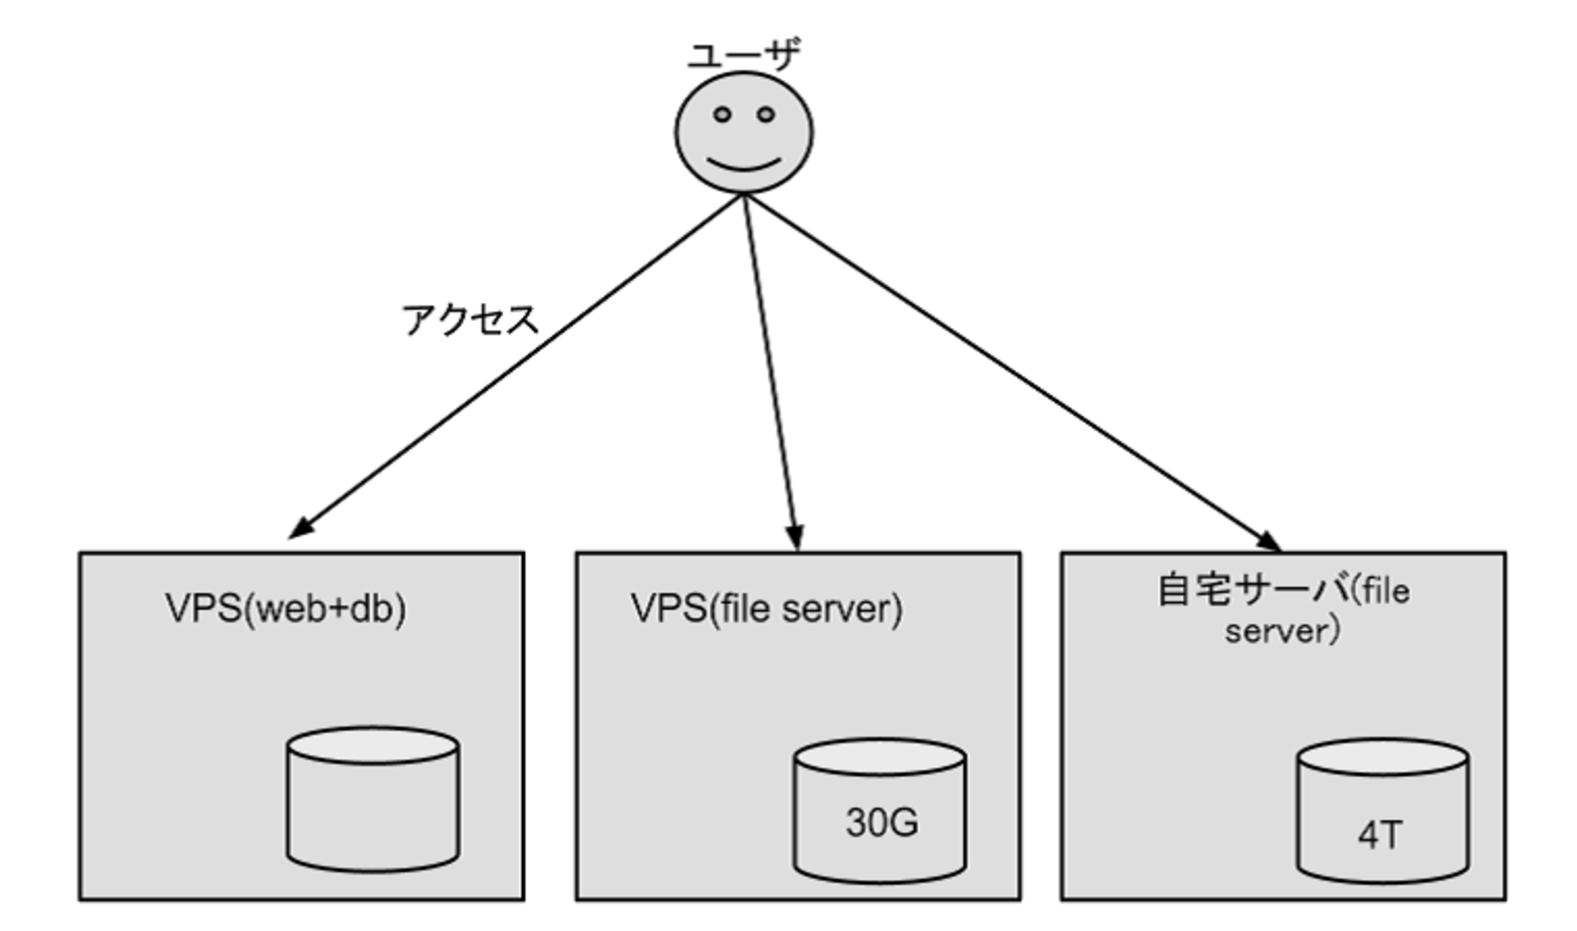
\includegraphics[width=120mm]{ijust3-mirror/img/mirror-servers.eps}
 \end{center}
 \caption{サーバ構成}
 \label{fig:mirror-servers}
\end{figure}

\subsubsection{負荷分散}
サイトオープン時は、自宅サーバ1台で運用していました。人気タイトルのゲームの体験版が出ると、自宅の回線の帯域が埋まってしまい、他のミラー素材も巻き添えでダウンロードしづらくなってしまう問題がありました。去年秋頃にVPSで広帯域のファイルサーバを用意し、アクセスが集中しそうなミラー素材をそこに転送する仕組みをつくりました。しかし、人気の素材が集中するとさすがにダウンロードしづらい状態になってしまいます\footnote{月末とか月末とか月末とか}

\subsubsection{アクセス制限と時限バッチ}
ミラー素材には、公開日時が決まっています。公開日時に手動でアップロードするのでは大変なので、事前にサーバ上へ置いておき、webサーバがアクセス出来無いパーミッションに設定しておきます。公開日時に時限バッチによってパーミッションが変更され、素材が公開されます。

\subsubsection{悪質ユーザとの戦い}
% IP limitconn

ユーザの中には、分割ダウンロードツールにより1クライアントから大量のアクセスを仕掛けてくる場合があります。会員制のサイトでは無いので、1つのIPから多くのアクセスが来た時は遮断する仕組みを入れて対応しています。%
分割ダウンロードツールを使っても、通信帯域がボトルネックになり、高速にダウンロードはできません。また、Webサーバのコネクションを食いつぶして、他のユーザへ迷惑が掛かります。

% 総転送量の制限
また、ミラー素材をかたっぱしからダウンロードしようとするユーザもいます。1日中、常にアクセスされている状態となると、やはり他のユーザへ迷惑となってしまうため、Webサーバのログを専用のDBサーバに格納し、IP毎に一定時間でダウンロード出来る総転送量を制限する仕組みを入れています。\footnote{実際に1日10回程度ありました}制限の閾値は一般のユーザには影響を与えない程度には大きく設定してあるので、通常に使用しているときは問題のないようになっています。

% TODO: 集計処理の話は要らない
%\subsubsection{集計処理}
%ミラーの依頼内容によっては、たまに、ダウンロード数を知りたいというメーカさんがいる。
%KELでは、各ミラーサイトへダウンロード数の集計処理は必須では無いとしている。が、集計も一応出来ると、よりメーカさんの期待に応えられる。

\subsubsection{アクセス数調査}
Google Analyticsを入れて、ユーザの動向も統計的に追うようにしています。
去年1年間を見ると、1日の訪問者数は1500~2000人程度です。しかし、サイト滞在時間が1分半程度と、ダウンロードが終わると皆直ぐに帰ってしまう傾向にあるのが分かります。

\subsection{東日本大震災の影響}
%
%- バックアップ超大事
%- 関東に半分程度のサイトが集中
%- 計画停電は自宅サーバの運営に支障

東日本大震災でメーカーの人から心配されたことがあります。自宅に置いてあったサーバに衝撃が加わり、ハードディスクが故障してしまいました。当時DBサーバは2台あって、レプリケーションをしてバックアップをとっていましたが、両方とも故障し、素材のファイルのパスなどの文字情報が消えてしまいました。すべて手打ちで入れていたので復旧が諦めきれず、HDDの復旧屋にたのんでデータは復旧しました\footnote{復旧費用は10万円くらいかかりました。データはMySQLのバイナリログから復旧したと記憶しています}。

壊れてしまったDBに入っていたデータが復旧するまでの間、新しいマシンを買ってきてサイトには「復旧中」の旨、表示をしていました。そんな中、計画停電に巻き込まれ、電源を確保することが出来ない状態になりました。ちょうどそのときにメーカーの人がサイトにアクセス。メーカーの人はミラーの依頼をしようとしていたところで、サイトが見られなくなっているため、被災したんじゃないかと心配したそうです。それではまずいとなり、急遽VPSを借りることになり、今の運用環境になりました。

% \subsection{ミラーサイトの管理者として思うこと}

% 案外、ゲームの情報は得られないです。噂で聞く頃にはユーザに広まっていたりします。あと、アフィリエイトは儲かりません。。。

\subsection{J-NODEについて}

最後に、J-NODEについて調べていたら、インターネットアーカイブ\footnote{http://web.archive.org}でこんな文章を見つけました\footnote{http://web.archive.org/web/20050404024212/http://www.j-node.co.jp/company.html}\footnote{J-NODEについてはwikipediaの「メイリッシュ」の項目をご覧ください}。

\begin{screen}
ネットサイド

近年ブロードバンドのスペックが広まる中、同じコンピューティング系事業を行うにあたってインターネット媒体を使わない理由はありません。当社では、インターネットを通じ普段ショップ越しでしか分からないエンドユーザー様の声を聞き、より充実した情報とサポートを実施すべく力を入れております。商品の映像やデータ、音声、そしてテキストといった多くの情報を分かり易く伝達することに挑戦しています。

 2002年からはエンドユーザー様と共同運営する形態という、企業の壁を超えた大容量ダウンロードサービスを展開し、より良い情報を提供しています。理解を得れたユーザー様に感謝すると共に、コミュニティという意味での共同運営が実現できた事は、多くのメリットを生み出しています。新しい手法で新しい勝機を生むネットビジネスを展開しております。

\end{screen}

当時、時代の最先端を行っていたと思います\footnote{ビジネスモデルが早すぎたんや…}。

\subsection{謝辞}
今回、初めて同人誌の記事を書かせて頂きました。書き始めた当初は壮大な計画を立てていたのですが、社会人として、仕事との両立の難しさも経験しながら、今回は雑誌の主テーマの技術系とは少し異なるライトな記事での執筆となりました。次回は、PostgreSQLと呼ばれるデータベース管理システムの検索実行処理について解説を書こうと思います\footnote{実は当初、このテーマで書こうと思っていました}。

記事の方針について右往左往しまして、多大なご迷惑をお掛けしました共同執筆者の皆様と、そして読者の皆様、最後にMagicMirrorのユーザの皆様へ、ここに記して謝意を表します。

\begin{thebibliography}{9} 
 \bibitem{fuzzy2_1} mirror.fuzzy2.com 「このサイトの歴史」 \url{http://mirror-f.fuzzy2.net/front/modules/pico/index.php?content_id=21}
 \bibitem{fuzzy2_2} mirror.fuzzy2.com 「KEL有志ミラーについて」 \url{http://mirror-f.fuzzy2.net/front/modules/pico/index.php?content_id=3}
 \bibitem{XES} XgameEloctronicStation 「御利用前にお読みください」 \url{http://www.xgamedata.com/index4.html}
\end{thebibliography}
